\chapter{Estado del arte}

\noindent\fbox{
	\parbox{\textwidth}{
		En este capítulo se analizará más a fondo la situación del problema, las soluciones ya realizadas, las herramientas que se pueden utilizar para realizar la solución, desde un punto de vista crítico.
	}
}

\section{Asistentes de Voz: Escuchar, procesar, responder}

Los Asistentes de Voz podrían definirse como un agente software que puede interpretar el habla humana y responder usando una voz sintetizada, según Matthew Hoy en su introducción a los Asistentes de Voz \cite{vaintroduction-matthewhoy}. 

En general, esperan a ser invocados por una palabra clave, tras lo cual graban lo que se dice y lo procesa, interpretándolo como un comando. Ese comando puede implicar desde responder con la información necesaria, pasando por interactuar con el dispositivo donde está instalado (por poner un ejemplo, pidiendo controlar elementos multimedia), hasta poder incluso manejarse con otros dispositivos dentro o fuera de su alcance.

\subsection{Una reseña histórica}
La historia de los Asistentes de este tipo está ligada como la aplicación de dos grandes campos de la Inteligencia Artificial: el Reconocimiento de Voz y la Síntesis de Voz.
\begin{itemize}
	\item El \textbf{Reconocimiento de Voz} persigue la conversión de una grabación de una voz a un texto con el mismo mensaje que el hablado
	\item La \textbf{Síntesis de Voz} busca justamente lo contrario: A través de un texto, lograr que una voz lo comunique.
\end{itemize}

Igualmente, profundizaremos en estos dos conceptos en sus secciones correspondientes, un poco más adelante.

En esta reseña histórica veremos los pasos relevantes en ambos campos hasta el primer Asistente de Voz.

\subsubsection{Experimentando con la voz}
Si bien la historia del reconocimiento de voz es más reciente, hace dos siglos se trataba de modelar el lenguaje según el movimiento del tracto vocal, dando así un paso en su síntesis.

La primera instancia de aparatos que usen la voz data de un juguete de 1918 denominado Radio Rex, el cual al decir el nombre de Rex un perro salía de su caseta. La cuestión en ello es que no reconocía la voz como tal, sino la vibración. Nada más tocar la caseta con un poco de fuerza o dar un golpe cerca de él, saltaba un contacto de cobre que accionaba un mecanismo.

No fue hasta 1950 que los Laboratorios Bell empezaron a hacer ciertos avances para reconocer la voz con Audrey \cite{audrey}. Era una máquina basada en una serie de relés que podía reconocer los dígitos del 0 al 9 y las palabras \textsc{Sí} y \textsc{No} con un 90\% de acierto. Sin embargo, ese aparato sólo podía reconocer ciertas voces y era enorme, con muchos cables y muy costoso. Se tenía ideado para automatizar el marcado en los teléfonos.

\subsubsection{Primeras aplicaciones del reconocimiento y síntesis de voz}
En 1930, los Laboratorios Bell crearon el \textit{Vocoder}, una máquina con un teclado que permitía analizar y sintetizar una voz electrónica, prometiendo ser una voz inteligible. Sin embargo, sonaba muy robótica y a veces no se entendía muy bien. Posteriormente evolucionó al \textit{Voder} \cite{voder}, que fue presentado en la Feria de Nueva York de 1939.

\begin{figure}[H]
	\centering
	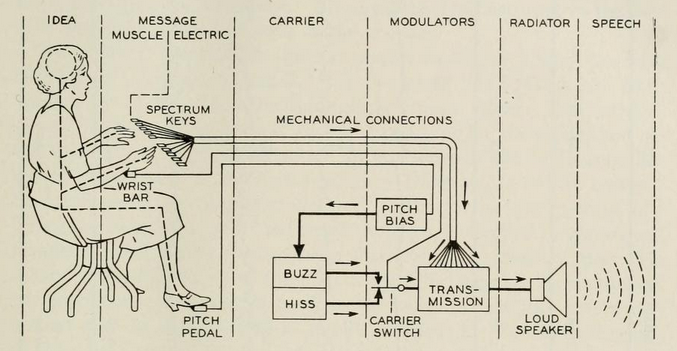
\includegraphics[width=\textwidth]{imagenes/Voder.png}
	\caption{Un esquema del \textit{Voder}. Extraído de \cite{voder}}
\end{figure}

La primera aplicación del reconocimiento de voz fue presentado por IBM en 1962. Con el nombre de \textit{Shoebox} \cite{shoebox}, era una calculadora capaz de reconocer 16 comandos (los dígitos, \textsc{Plus}, \textsc{Minus}, \textsc{Subtotal}, \textsc{Total}, \textsc{False} y \textsc{Off}). Su salida se emitía sin embargo en una impresora.

En 1961, el Doctor J.L Kelly usó un IBM 704 para sintetizar voz a través de un ordenador, cantando una canción en compañía de una orquesta. A partir de ese punto se ha ido trabajando en alas de una voz más natural que se pudiera lanzar con altavoces más pequeños.

En 1972, en el DARPA, se culminó un sistema más complejo de Reconocimiento de Voz denominado \textit{Harpy} \cite{harpy}, el cual permitía reconocer 1000 palabras e incluso sus combinaciones con tal de crear oraciones y sentencias.

En los 90, se empezó a vender programas software como \textit{Dragon Dictate} \cite{dragon-dictate}, que permitía reconocer bastantes palabras y que se distribuía de forma comercial al público, aunque el monto a gastar por entonces era de 6000 dólares.

\subsubsection{Los primeros Asistentes Virtuales: el don artificial del habla}

El campo de los Asistentes Virtuales ha sido basado en texto durante bastante tiempo, donde a través de un globo podías leer sugerencias y consejos (como ejemplo podemos poner a Clippy, incorporado en 	Microsoft Office 97). Pero hubo dos grandes eventos que dieron pie a la actualidad de los Asistentes de Voz, solapando la los años más recientes. En general, la década de los 2010 ha sido la que estamos continuando actualmente.

\begin{itemize}
	\item Por una parte, el equipo \textit{DeepQA} de IBM \cite{deepqa} se dedicó desde 2004 a hacer un sistema que pudiera responder cualquier pregunta hablada. Este fue más conocido por ganar en simulacros de \textit{Jeopardy} contra campeones de ese programa en 2010 y 2011.
	\item Por la otra, la popularización de los \textit{smartphones} con los iPhone de Apple y la compra de Siri para su posterior mejora, dio la popularidad de los Asistentes Virtuales de Voz que conocemos actualmente.
\end{itemize}

\subsection{En la actualidad...}
Esta era es el apogeo de los Asistentes Virtuales, que están empezando a desarrollarse en multitud de formatos por parte de varias compañías conocidas. En esta parte hablaremos de algunos de ellos a modo introductorio, aunque en el Análisis hablaremos en detalle y analizaremos competitivamente sus habilidades.

\subsubsection {Aplicaciones populares}
Hoy en día, las empresas más importantes tienen una instancia de Asistente Virtual por voz. Comentemos algunas de ellas:

\begin{itemize}
	\item \textbf{Apple Siri} \cite{siri} Como se comentó previamente, fue el resultado de la compra de esa aplicación, la cual se integró en el iPhone 4S para darle distintivo a sus dispositivos, presentándose el 14 de Abril de 2011. Con el tiempo se fue extendiendo a los aparatos de Apple, formando parte de su ecosistema.
	\item \textbf{Google Now} Al principio fue diseñado como un sistema de tarjetas que iba aprendiendo de las búsquedas e información del usuario para dar información relevante, pero este no respondía con voz. Posteriormente evolucionó a \textbf{Google Assistant} \cite{google-assistant} en Mayo de 2016, primero como parte de una app y extendiéndose de forma análoga a Siri en los dispositivos del ecosistema de Google y Android, siendo este software el que lo enmarca en esta lista.
	\item \textbf{Amazon Alexa} \cite{alexa} Alexa fue presentada en Noviembre de 2014 para dispositivos Echo. Debido a la gran infraestructura que posee esta multinacional en cuanto a servidores y servicios de \textit{cloud} se refiere, gran parte de ese procesamiento pasa por esas infraestructuras. Además permite hacer aplicaciones (o \textbf{skills}) para que terceros puedan integrarse con este Asistente. Actualmente ha sido integrado en multitud de dispositivos incluso fuera de su ecosistema.También se está ofreciendo como un \textit{SaaS} (\textit{Software as a Service}) para poder integrarlo donde se pueda, además de ciertos plus como voces de famosos.
	\item \textbf{Microsoft Cortana} La respuesta por parte de la empresa de Bill Gates ante el boom del tema a discutir, y tomando la inspiración de una de los personajes más icónicos de \textit{Halo} (uno de los juegos más famosos de la consola de la compañía, \textit{Xbox}), fue presentada en una conferencia de la empresa en Septiembre de 2014. Con la llegada de Windows 10, este asistente llegó integrado. Hay constancia de dos versiones para Android y iOS, pero sólo en inglés. A día de hoy, se están redirigiendo los esfuerzos del proyecto de cara a la productividad empresiaral con la línea de Microsoft 365 \cite{cortana}.
\end{itemize}

Además de estos, hay un montón más de ellos. En algunos casos, se crean por la falta de soporte de alguno de las empresas más grandes (por ejemplo, \textbf{Huawei Celia} \cite{huawei-celia} fue desarrollado por las restricciones de Estados Unidos). En otros, por tener otras alternativas con filosofías como el \textit{FOSS}, del cual hablaremos posteriormente. Un ejemplo de ello es \textbf{MyCroft} \cite{mycroft}, que asegura la privacidad de la información y la apertura de su código, además de ofrecerse como una alternativa ligera en cuanto a recursos.

Posteriormente haremos un análisis competitivo de estas opciones a fin de comparar su funcionamiento y prestaciones, para hacernos una idea general de posibles mejoras.


\subsubsection{Un sinfín de formatos}
Hoy en día, podemos encontrarnos estas aplicaciones casi en cualquier lado. Si bien en un principio estaba pensado para smartphones, enseguida fue adaptado a otros aparatos.
Una de las propuestas fue con Amazon y su asistente Alexa, que fue embebida en un dispositivo sin pantalla llamado Echo \cite{echo}. Sólo dispone de altavoces, micrófonos, una luz para saber si escucha y se podía conectar con el teléfono para poder insertar las contraseñas pertinentes. Posteriormente se hizo una versión que tenía una pantalla para mostrar algunas cosas.
Gracias a la variedad de versiones de ese producto, se permite tener uno de esos Asistentes por precios más o menos caros, con calidades más o menos Premium.

En general, los movimientos en estas aplicaciones tienden a comenzar en un pequeño sector el cual trata de expandirse para formar parte de la experiencia de un ecosistema donde se ha desarrollado.

\begin{figure}[p]
	\centering
	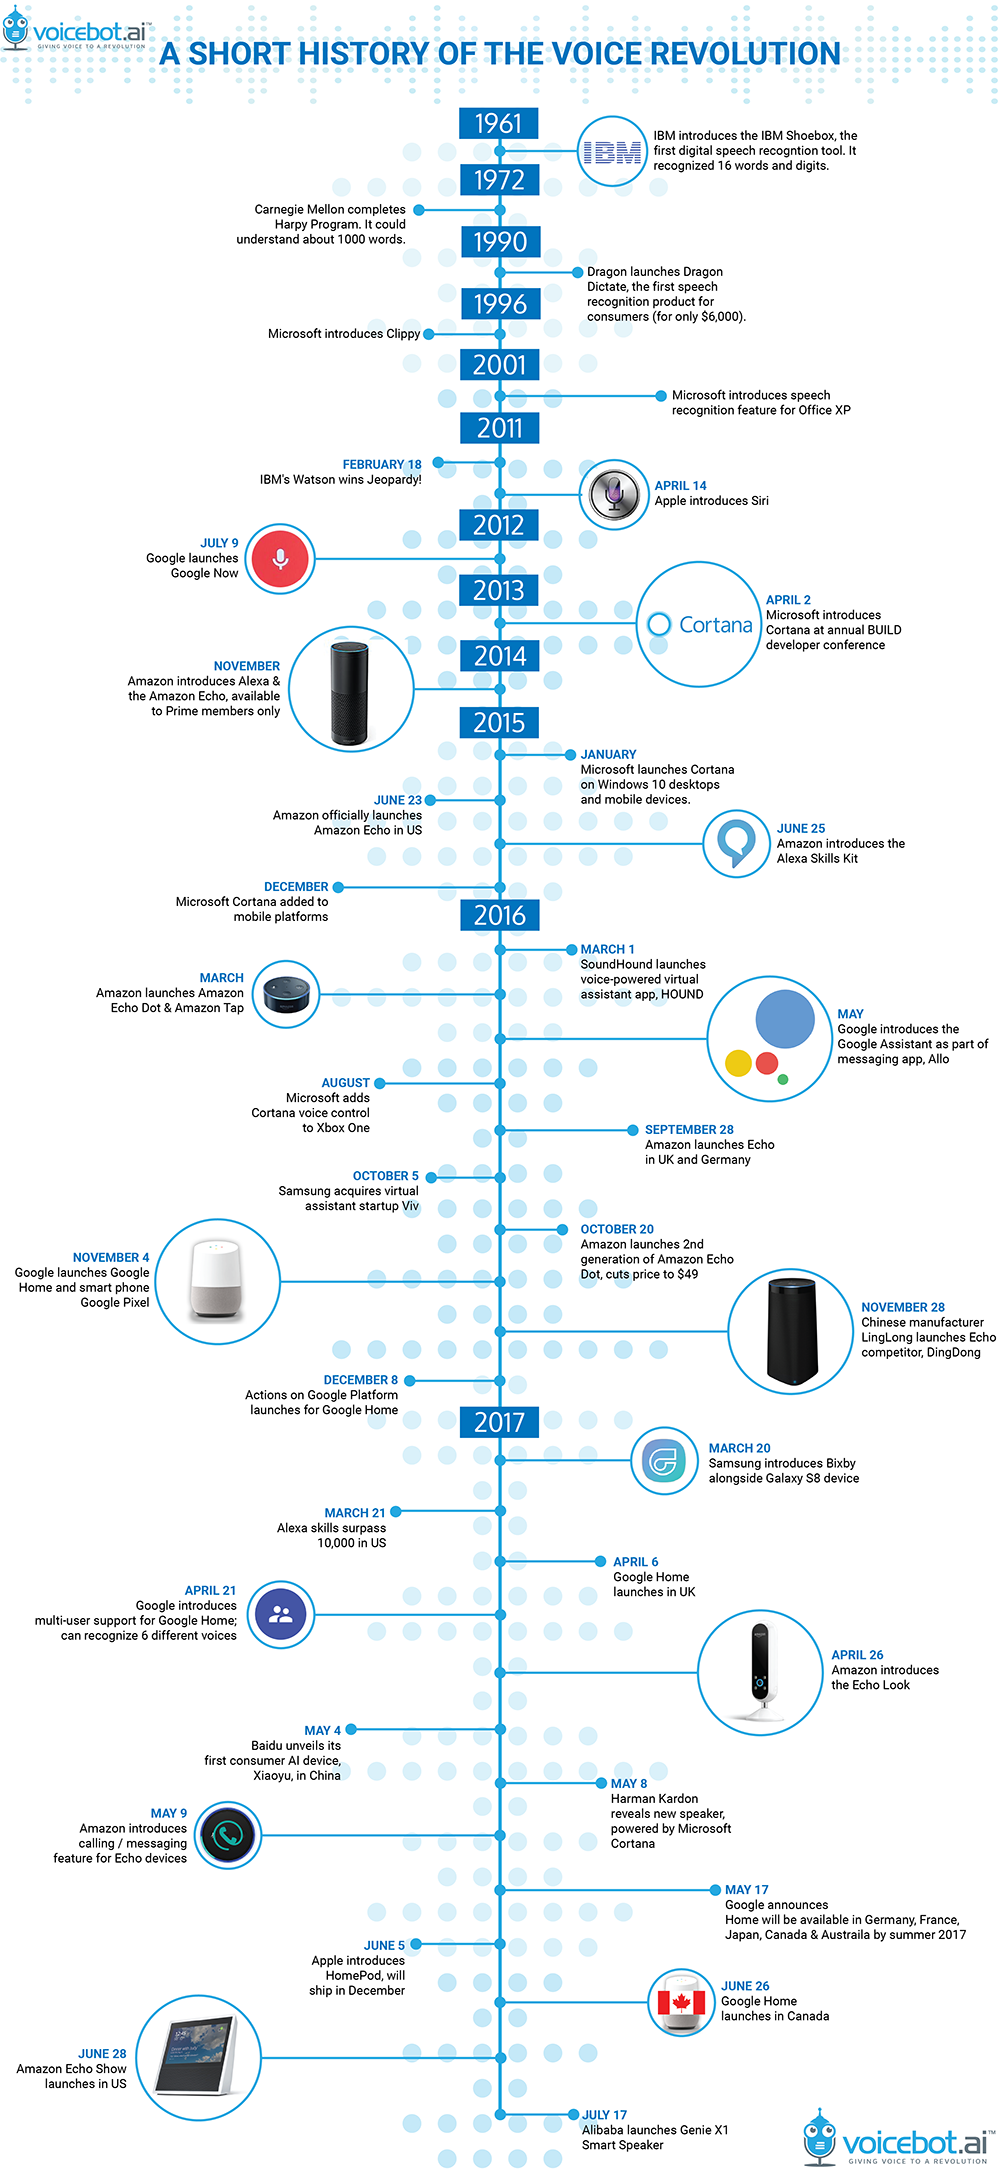
\includegraphics[height=0.98\textheight]{imagenes/Timeline_VA.png}
	\caption{Una timeline con algunos de los eventos más importantes en el área. Extraído de \cite{va-history}}
\end{figure}

\subsubsection{Las ventajas}
 \begin{itemize}
 	\item Una de las más notorias, como hemos visto, es que podemos tener uno de ellos en cualquier sitio. Como hemos comentado antes, desde dispositivos dedicados como los altavoces inteligentes, pasando por ordenadores y \textit{smartphones}, hasta aparatos del Internet de las cosas como \textit{Smart TVs}.
 	\item La información se está solicitando y recibiendo usando la voz, por lo que no es necesario usar las manos o la vista (como hemos comentado en la Introducción), por lo que uno de los usos sería para personas ciegas o con diversidad motora (véase, por ejemplo, la cuadriplejía). Pero además es un punto de acceso para aquella gente que tampoco sepa o pueda leer o escribir, gracias a cómo se puede comunicar la información.
 \end{itemize}
\subsubsection{Las desventajas}
	\begin{itemize}
		\item La más importante está relacionado con la seguridad y privacidad de lo que se usa en ello. Matthew Hoy \cite{vaintroduction-matthewhoy} comentaba en su Introducción a los Asistentes Virtuales que se podría preguntar al propio asistente por información de aquellas cuentas e integraciones que tenga conectadas, o pedirle que le haga tareas.
		
		Como adición a ese comentario, decir algunas de ellas no reconocen exactamente de quién es la voz, por lo que sintetizar la voz para un comando o tener el altavoz de algún dispositivo cerca de este e invocar al software durante una llamada podría ser suficiente para que el Asistente funcione y ejecute lo que se quiera.
		
		Como extra, tengamos en cuenta que uno de los componentes principales de un Asistente de Voz es un micrófono. Aunque conceptualmente sólo sirva para cuando se le llama explícitamente, este igualmente está grabando mientras espera a que se diga su palabra de invocación (o \textit{trigger word}). Como consecuencia, puede generar cierto alarmismo por ese hecho y, en el caso de que alguien pudiera lograr usar ese micrófono para obtener las grabaciones con otros propósitos, generar una brecha de privacidad que podría ser explotada.
		
		\item Si bien se han hecho progresos en los campos del \textit{Speech Recognition} y el \textit{Text-To-Speech}, no son perfectos. Por lo tanto, es posible que ante una petición el comportamiento puede ser un poco indeterminado según la tolerancia del Reconocedor, su entrenamiento y cómo el usuario se exprese.
		
		Por otra parte, la voz que se sintetiza puede llegar a resultar algo robótica, aunque se tratan de hacer esfuerzos en que se intente ser más natural. La otra opción, si se quisiera ser totalmente natural, sería que alguien grabara las voces y estas se reproduzcan, pero además de resultar algo tedioso ya que pueden haber muchas respuestas por grabar, ocupan mucho espacio, algo no muy deseable.
	\end{itemize}

\section{Fundamentos de los Asistentes de Voz}
Por lo analizado a través de la historia y la situación actual podemos intentar extraer un marco teórico que recogería todos los elementos de los Asistentes de Voz y cómo se combinarían para formar algo.

\subsection{Una idea intuitiva}
Para empezar, podríamos empezar con lo que haría un \textit{software} convencional. Se alimenta con una serie de datos, se procesa y acaba saliendo otra serie de datos. Si representáramos ese concepto en un diagrama, tendríamos lo siguiente:

\begin{figure}[H]
	\centering
	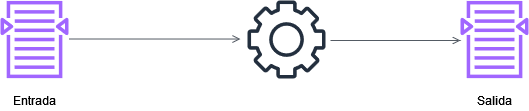
\includegraphics[width=\textwidth]{imagenes/DiagramaBase.png}
	\caption{Diagrama básico de un software. De elaboración propia.}
\end{figure}

Los datos que recoge, en nuestro caso, son voces. Por el otro extremo, lo mismo. Podríamos actualizar nuestro diagrama con esa salida.

\begin{figure}[H]
	\centering
	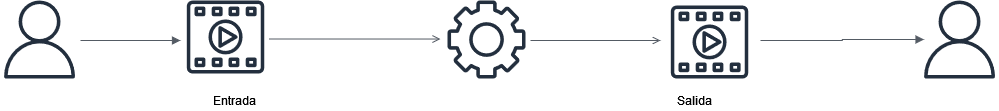
\includegraphics[width=1.1\textwidth]{imagenes/DiagramaDatos.png}
	\caption[Diagrama modificado.]{Diagrama modificado. Nótese que en vez de documentos se usa multimedia. De elaboración propia.}
\end{figure}

Esas voces que se recogen no se generan solas. En el caso de la recogida, es un usuario quien habla a través de un micrófono para grabar esa voz que podrá procesar posteriormente. En el otro lado, esa voz se reproducirá a un altavoz. Esos procesos de grabación y reproducción tienen ya de por si su propia lógica intermedia para poder procesarlos. Con esta nueva información, el diagrama quedaría de la siguiente forma:

\begin{figure}[H]
	\centering
	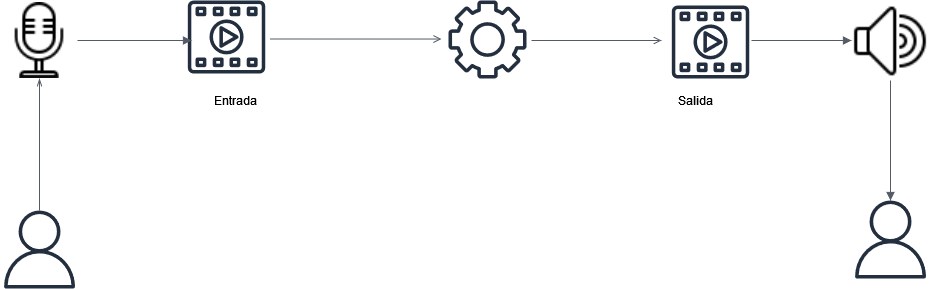
\includegraphics[width=1.1\textwidth]{imagenes/DiagramaIO.png}
	\caption[Diagrama con E/S.]{El mismo diagrama que el anterior, pero señalando las Entradas y Salidas. De elaboración propia.}
\end{figure}

Ahora tenemos otras dos cuestiones sobre esos archivos de audio.
\begin{itemize}
	\item ¿Cómo puede entender \textbf{qué está diciendo esa voz}?
	\item ¿Cómo se crea \textbf{el audio de la respuesta} a partir de un texto?
\end{itemize}
La respuesta a esas dos preguntas resulta ir en dos campos respectivos de la Inteligencia Artificial: el \textbf{Reconocimiento} (o \textit{\textbf{Speech Recognition}}) y la \textbf{Síntesis de Voz} (conocido más como \textbf{\textit{Text-to-Speech}}). 

Por lo tanto, se crea una lógica para poder hacer esas conversiones, de forma que podríamos hacer que el sistema nos escriba qué ha entendido (reconociendo esa voz) y que ``lea'' la respuesta con lo que le hayamos escrito (sintetizando la voz). De todas maneras, hablaremos de ello más adelante. Podríamos actualizar el diagrama resultando en esta figura.

\begin{figure}[H]
	\centering
	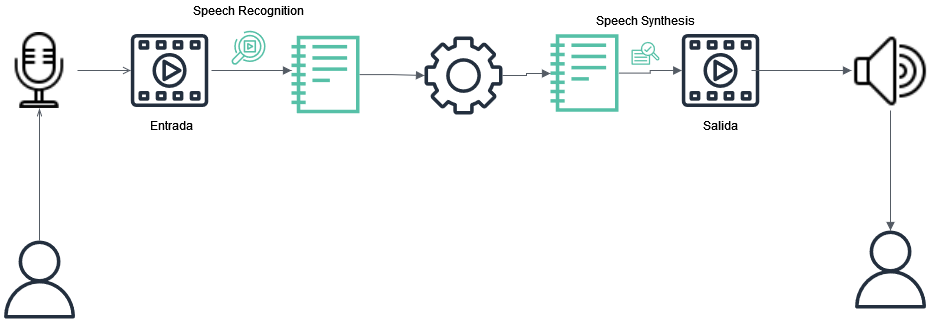
\includegraphics[width=1.1\textwidth]{imagenes/DiagramaTTS_SR.png}
	\caption[Diagrama con TTS/SR]{El diagrama anterior pero señalando las interacciones con el Speech Recognition y el Text-To-Speech (o Speech Synthesis). De elaboración propia.}
\end{figure}

Por último, la lógica que hay entre lo que se ha dicho y lo que tiene que leer la máquina debería poder procesar esa frase, buscar si sigue algún patrón o usa alguna palabra de relevancia (como ``Reproduce'', ``Canta'' o ``El tiempo en una ciudad''), y dar una respuesta que se pueda leer. Por lo tanto, el diagrama final a modo conceptual podría darse como la de la siguiente figura: 

\begin{figure}[H]
	\centering
	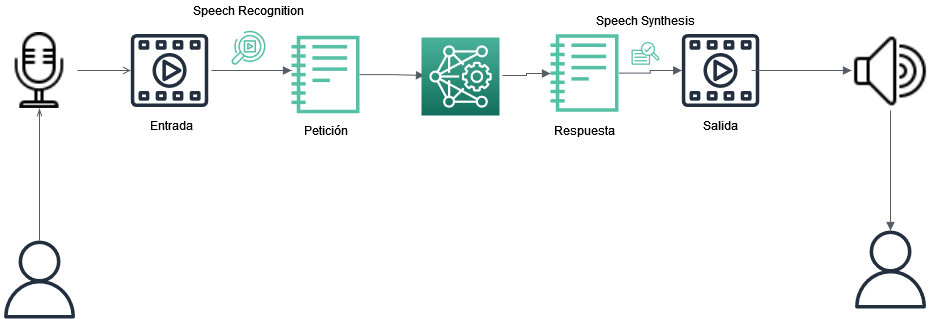
\includegraphics[width=1.1\textwidth]{imagenes/DiagramaIntuitivo.png}
	\caption[Diagrama intuitivo final.]{Diagrama resultante. Nótese que la lógica en verdad es un proceso de relacionar conceptos. De elaboración propia.}
\end{figure}

En resumen, podríamos decir que un Asistente de Voz consta a nivel \textit{hardware} de un ordenador con un micrófono o entrada de audio y un altavoz o salida de audio.

Sin embargo, a nivel \textit{software} necesitaríamos:
\begin{enumerate}
	\item Un módulo para gestionar las \textbf{grabaciones del micrófono} que diga cuándo grabar, cuando parar, y que guarde la grabación para poder trabajar con esta. Esta nos devuelve un audio
	\item Una parte para hacer \textbf{Reconocimiento de Voz} a través de esa grabación. Nos devuelve el mensaje de ese audio.
	\item La \textbf{lógica principal} del programa, que mira el mensaje y responde con otro.
	\item Una parte para poder hacer \textbf{Text-To-Speech}, convirtiendo la respuesta en otro audio.
	\item Un módulo para poder \textbf{reproducir ese audio} con la respuesta a través del altavoz, que cargue el archivo y lo reproduzca.
\end{enumerate}

\subsection{El reconocimiento de voz}
En la documentación sobre el tema, IBM \cite{sr-definition} define el Reconocimiento de Voz o \textit{Automatic Speech Recognition} (ASR) como la capacidad de un programa de procesar el habla y convertirlo en un texto escrito legible, que puedan entender también las máquinas para el posterior procesado de la información.

Para poder reconocer esa voz, se necesita primero separar ese sonido en pequeños fragmentos que pueda comparar con un Modelo Acústico (es decir, un conjunto de sonidos pequeños que se conoce lo que significa), de forma que se pueden asociar los del audio enviado con estos para buscar similitudes. Con ello, se busca en un Modelo del lenguaje (un conjunto de letras o combinaciones de estas asociadas a ese sonido) qué palabras quieren decir, y las compara para dar un porcentaje de acierto. Finalmente devuelve un texto o varias versiones de un texto según las opciones que haya ido observando.

Uno de los grandes retos en este campo viene porque no todos tenemos la misma voz, y por lo tanto si bien los Modelos Acústicos pueden reconocer muchas de ellas, no puede con todas, y es imposible tener todas las voces almacenadas. por lo tanto, se han pensado en varias maneras de abordar ese problema a través del Aprendizaje Automático. Mencionaremos algunas de ellas en estos epígrafes a un nivel introductorio. \cite{sr-methods}

\subsubsection{Modelos de mezcla Gaussiana} 
Una primera tarea para abordar este campo sería usar la probabilidad de que el sonido coincida con lo que tiene en su modelo, pudiendo así saber qué sonido tiene cada uno.

Si representáramos en una gráfica dos variables (como el fonema y el tiempo), podríamos ver que esos puntos se podrían agrupar en \textit{clusters} que se acercan a ese fonema para dar con la media de ellos y sacar el que más se parezca al resultado, haciendo así una clasificación de los sonidos. Eso es precisamente cómo funciona el modelo de mezcla gaussiana.

Un modelo de mezcla Gaussiana \cite{gaussiana} es un modelo probabilístico que asume que todos los puntos a analizar se han generado a través de varias distribuciones gaussianas juntas (una cantidad $K$ de ellas). Por lo tanto, un punto en el plano puede estar cerca de un punto intermedio de esos $K$ que representa una de las distribuciones que se han mezclado, dando a entender que ese punto sea más probable de pertenecer a esa distribución que a otra.

\subsubsection{Modelos ocultos de Markov} 

El propio hecho de intentar predecir qué va a decir alguien es un tanto arduo, ya que el mensaje que vas a comunicar puede ir completándose durante el tiempo que se está hablando. Podríamos decir entonces que el hecho de hablar es dar una cadena donde nos vamos enterando del mensaje por la secuencia de sonidos aleatorios, generando fonemas que se unen y comparan con los modelos para encontrar las palabras.

Al final, podríamos darnos con esta serie de condiciones:
\begin{itemize}
	\item Tenemos un tiempo que podemos cuantificar discretamente : $ t \in \{1,2,3...\} $
	\item Cada instante tenemos unas variables aleatorias que podemos o no observar (por ejemplo, la frecuencia del sonido o la letra que intenta decir)
	\item Las relaciones entre los estados de esas variables según el tiempo sólo dependen del estado anterior (en nuestro caso, si se intenta decir \textit{mesa}, se debería escuchar primero la letra \textit{m}, luego entender \textit{me}, y así sucesivamente)
	\item Los estados finales que puede tomar cada sonido al final se pueden relacionar con una letra o conjunto de ellas, que si bien es un conjunto grande, al menos es finito.
\end{itemize}

Esto podría ser por lo tanto un caso de aplicación de un \textbf{Modelo Oculto de Markov}\cite{modelo-markov}, donde tenemos por una parte una variable aleatoria de estado que no se puede observar directamente (cómo en nuestro caso la letra o fonema que va a decir) y por la otra una variable que sí podemos observar directamente (por ejemplo, si grabamos ese sonido y sacamos su representación de las frecuencias).

Este modelo posee dos propiedades que tienen cabida en el contexto que presentamos:
\begin{itemize}
	\item \textbf{Propiedad de Markov} En cada instante, el estado sólo depende del estado anterior. En nuestro caso, si en un instante $t$ se tiene la alta probabilidad de que un sonido se asocie con una consonante, en la siguiente ($t+1$) habría una gran probabilidad de que fuera una vocal, visto lo anterior.
	
	\item \textbf{Independencia de las percepciones} En cada instante, lo observado sólo depende de ese instante. Si en el caso del Reconocimiento de Voz tuviéramos en cuenta el sonido de antes, sería muy difícil saber qué fonemas suenan en cada momento para poder asociarlos correctamente, dando lugar a errores de comprensión.
\end{itemize}

Así, podríamos ver ese modelo como una especie de máquina de estados basado en una serie de probabilidades de que cambie de un estado a otro según lo que se observe.

\subsubsection{Redes neuronales en el ámbito del Speech Recognition}
Las redes neuronales son en esencia nodos con varias entradas que tienen asociados un peso o importancia a tener en cuenta, que se van ajustando según las conexiones en un grano más fino y se concentran en un resultado final que activa o desactiva.

De esta forma, primero se entrena la red neuronal con una serie de datos que se saben qué resultado tienen para poder ajustarlo; y una vez entrenado, ya se puede dejar con datos que no se han probado.

\subsubsection{Frameworks y librerías}

Hoy en día hay servicios a través de la nube que ofrecen APIs que permiten el reconocimiento de voz, además de softwares y librerías que permiten hacerlo de forma local, aunque al estar orientado a modelos embebidos tienen un reconocimiento más limitado que a través de servidores que pueden almacenar más sonidos y relaciones.

En cuanto a servicios en la nube podemos destacar \textbf{IBM Watson} \cite{ibm-sr}, \textbf{Amazon Transcribe} \cite{amazon-transcribe} o \textbf{Google Cloud} \cite{google-stt}, los cuales usan sus soluciones para ofrecer una API que permite obtener el audio a partir de una serie de instrucciones contenidas en una biblioteca o en varios endpoints.

Sobre las soluciones más limitadas pero locales, podemos hablar de \textit{Vosk API} \cite{vosk}, que tiene modelos de 50 MB para idiomas como el Español, el Inglés o el Catalán.


\subsection{La síntesis de voz}
Si el reconocimiento de voz trata el procesamiento del habla para extraer un texto, la síntesis de voz sería lo contrario, la producción artificial de ese habla \cite{tts-definition}. 

Para ello se usan como base los grafemas (aquellas letras y grupos que se pronuncian de una manera). De esa forma, se separa el texto en dichos grafemas, tras lo cual se asocian esos grafemas a sus correspondientes sonidos o fonemas asociados, entonando así cada palabra, frase y finalmente leyendo el texto.

Eso sí, de forma similar al Reconocimiento de Voz, tienen un Modelo para asignar los fonemas a sus grafemas. Aunque en este caso se simplifica el modelo acústico ya que se usa una serie de sonidos predeterminados para darle una voz al resultado.

Uno de los grandes retos que se ha ido viendo mejoría es la naturalización de la voz que sintetiza. Si bien ha habido una mejora desde su creación y aún va evolucionando año tras año, todavía queda camino para llegar a una voz que no pudiéramos etiquetar como robótica.

Al ser el Reconocimiento y la Síntesis de Voz procesos contrarios, se pueden emplear los mismos métodos para hacer una u otra cosa.

En cuanto a soluciones ya implementadas, por parte de la nube tanto Amazon \cite{polly} como IBM \cite{ibm-tts} y Google \cite{google-tts} también tienen su TTS, y si hablamos de software local tenemos opciones como Festival \cite{festival} o las voces preinstaladas en Microsoft, o Siri en caso de los Mac.
 

\subsection{La lógica}

La lógica del proyecto se puede parecer al de un chatbot de texto, el cual tiene como unidad básica las palabras, que se unen para poder encontrar sentencias o patrones que puede usar para asociarlas con una respuesta y así enviarlo al usuario.

La primera aproximación para tener ese bot funcionando sería ir comprobando que lo que se envíe tenga una palabra clave que pueda buscar para saber si debe actuar \cite{chatbots-architecture}. Pero las respuestas serían bastante estáticas.

Una evolución de ello es que reconozca varias palabras en conjunto, o que admita múltiples palabras para llegar al mismo resultado, dando así un poco más de responsividad ante varias maneras de hacer la misma petición, pero no arreglaría lo primero.

Podríamos entonces añadirle algunas peticiones que requieran de algo variable, como preguntar por el tiempo en una ciudad. De esta manera, las respuestas son más personalizadas para cada uno. El problema con esta iteración es que hay que saber dónde buscar esa información, pero hoy en día está solventado ya que gracias a la aparición de APIs y conexiones con Bases de Datos se pueden enriquecer esas mismas respuestas.

Estas ideas han dado lugar a algunos lenguajes de marcado basados en \textit{pattern matching} que permiten realizar esas distinciones para dar respuestas. Podemos listar algunas de ellas:
\begin{itemize}
	\item \textbf{AIML (\textit{Artificial Intelligence Markup Language})} \cite{aiml} Es un lenguaje basado en XML que permite realizar algunas cosas básicas como guardar información básica, usar datos descritos en el patrón para devolverlos y decir respuestas aleatorias. Fue pensado para usarse en otro programa llamado \textit{AliceBot}, pero hay programas que permiten realizar el \textit{parsing} de documentos de este tipo.
	
	La base de AIML son las categorías, que dentro tienen patrones que escriben los usuarios y plantillas que devuelven los bots.
	
	\item \textbf{RiveScript} \cite{rivescript} Basado en AIML, pero en vez de usar los bloques de XML utiliza unos pocos símbolos.
	
	\item \textbf{ChatScript} \cite{chatscript} Basado en el Procesamiento del Lenguaje Natural, este lenguaje de scripting utiliza una serie de reglas para ejecutar las respuestas. Además permite hacer llamadas HTTP a servidores.
\end{itemize}

Aparte de esta aproximación, podríamos usar un algoritmo para buscar a partir de una serie de datos sobre qué se habla, o usar una serie de redes neuronales como el \textbf{NLP} (\textit{\textbf{Neural Language Processing}}) con tal de que esos patrones se estudien para dar después con unos nuevos, usando para ello \textit{Machine Learning} \cite{chatbots-architecture}

\section{Software Libre, Software de Código Abierto y Licencias}
El software libre y sus licencias \cite{gplv3} ha permitido llevar a cabo una expansión del aprendizaje de la informática sin precedentes. 

Como se ha comentado en el primer capítulo, sirve como respuesta a la colisión de la protección de las propiedades intelectuales de las empresas contra los derechos de los usuarios por los cuales, con una copia adquirida, no puedan emplear algunas herramientas para poder preservar el producto que ha adquirido de ellos. Además permite, igual que en la ciencia, compartir el conocimiento para construir a partir de ahí todo lo necesario.

Se ha llegado a un punto en la actualidad donde muchas de las herramientas más populares tienen una alternativa de software libre o ,al menos, de código abierto.

\subsection{¿Desde cuándo existe?}
La historia del software libre empieza más allá de que se acuñara ese término \cite{foss-history}. En los años 60, era muy común que aquellos con la suerte de tener un ordenador trataran de facilitar el código de sus programas entre ellos. De hecho,las compañías que manufacturaban esos ordenadores no hacían la separación comercial del software dentro de las capacidades del computador.

Ya en la década de 1970, empezaron a surgir empresas que comerciaban software de forma explícita, de forma que fuera compatible con hardware diseñado por otros con el objetivo de lucrarse con estos programas. Para limitar lo que podían hacer con esas aplicaciones, estas compañías ponían trabas a la hora de compartir, modificar y estudiar su producto.

Como respuesta a ellos, y sobre todo en los centros universitarios como \textit{Berkeley} o \textit{Massachussets}, se formaron grupos académicos que distribuían sus programas de forma libre, siendo éstos un esbozo de lo que se conocen actualmente como grupos \textit{FOSS} (de \textit{Free and Open Source Software}) 

Los hitos más relevantes en esta línea temporal fueron el desarrollo del Proyecto GNU de Richard Stallman, quien  sentó las bases de la iniciativa del Software Libre con sus 4 libertades \cite{fsf-philosophy} que permiten el uso, modificación, compartición y estudio de aquel software que estuviera forjado con esa filosofía. Empezando como un proyecto que perseguía hacer un Sistema Operativo similar a Unix, sirvió para realizar montones de utilidades que seguimos usando aún a día de hoy, gracias a la aparición del segundo hito relevante.

Este segundo hito no es ni más ni menos que la creación de Linux por el finlandés Linus Torvalds, que si bien al principio no estaba puesto como Software Libre, en su versión 0.12 \cite{linux-releasenotes0.12} se cambió a tal, lo que fue del agrado del proyecto GNU. Junto con la propagación del nuevo SO y la adaptación de las herramientas de GNU a este, se consolida una base sobre la que empresas y fundaciones dedicadas al \textit{FOSS} realizan compilaciones y variaciones sobre el núcleo dando lo que se conocen como \textit{distros}.

\subsection{¿En qué beneficia liberar el código?}
En una charla sobre Software Libre se discutió este punto \cite{osl-charla-liberatucodigo}, llegando a 4 grandes beneficios que enumeraré a continuación:

\begin{enumerate}
	\item \textbf{Esforzarse en cumplir con buenas prácticas de desarrollo} Al ser un código que todo el mundo va a ver, puede servir para acostumbrarnos a tomar buenas prácticas de desarrollo, como el Test Driven Development, seguir patrones y arquitecturas de diseño software
	\item \textbf{Generar una comunidad y/o participar en otras} Al liberar el código, por una parte colaboras en el mundo del software libre ofreciendo un nuevo proyecto que pueden estudiar y usar como alternativa a otros; y por otra generar una comunidad alrededor del proyecto a través de aportes, discusiones, documentación...
	\item \textbf{Añadir un proyecto al portfolio personal} Siendo esta la parte más individualista de las ventajas, tener un proyecto en una forja como \textit{GitHub} permite a las empresas ver cómo trabajas y qué cosas te interesan de cara al mundo laboral y empresarial.
	\item \textbf{Generar un ejemplo a la comunidad de desarrolladores} Al liberar el código das una condición de transparencia a todo lo que se hace, cosa que viene bien en instituciones públicas como Universidades o Empresas asociadas al Estado.
\end{enumerate}



\subsection{El curioso mundillo de las Licencias y sus restricciones}

Uno de los puntos más interesantes del Software Libre es que para poder proteger y asegurar que las condiciones de ésta se cumplan, hayan recurrido a crear un entorno legal que sirva de punto de referencia sobre la que partir y ayudar al desarrollo de proyectos dentro de este marco. \cite{foss-marcojuridico}

\subsubsection{Detallando el marco legal de las Licencias}
Las licencias son, como bien hemos dicho previamente, un contrato entre la persona que lo crea y el desarrollador que quiere aplicarlo en su proyecto. Esto da lugar a una serie de condiciones que deben cumplir ambas partes con tal de llegar a un punto donde ambas partes estén de acuerdo. En general se aplican licencias genéricas hechas por organismos reconocidos como la \textit{Free Software Foundation} o \textit{Creative Commons}, pero si se sabe de legislaciones y cumplen con la finalidad de poder estudiar y usar sin muchas restricciones, se podría realizar y usar.

Vamos a hablar de algunas de las licencias más comunes usadas en el ámbito del Software Libre e incidiremos en el punto de la creación de licencias.

\subsubsection{Free Software Foundation}
Creadas en 1989, se crearon las licencias GPL con el objetivo de proteger el software del proyecto GNU de que terceros hicieran algunas modificaciones que explotaran en un software privativo.

Si bien al principio fue una licencia popular, este llevaba a que encontraran una serie de brechas en la descripción de la licencia. Estas eran \cite{gplv3-changelog}:
\begin{itemize}
	\item \textbf{Tivoización} En honor a los aparatos de recepción de vídeo TiVo, es el hecho de que el software con posibilidad de modificación no se pudiera instalar en esos receptores ya que el hardware no lo soportaría.
	
	\item \textbf{Compatibilidad con el Affero GPL} debido a que no había cláusulas sobre el software en red.
	
	\item \textbf{Cláusula contra las represalias de patentes} Si bien en España y la mayoría de países se protege el software a través de los derechos de autor, en países como EEUU o Japón se puede patentar, y con esta versión se persigue que haya un amparo legal contra quienes intenten patentar el software libre y usen esas herramientas legales a quienes deseen modificarlo. De esta manera se hace un control de daños, ya que no se puede como tal evitar patentar versiones modificadas de un software libre.
	
	\item \textbf{Protección para herramientas contra el DRM} de forma que se pueden publicar programas que jueguen con la protección de los derechos de autor sin romper leyes de ese tipo, como el DMCA estadounidense.
	
\end{itemize} 

Todo ello se resolvió con la versión 3 de sus licencias. \cite{gplv3-changelog}

Por parte de la FSF, se han creado 3 licencias que se usan popularmente en este mundillo:

\begin{itemize}
	\item \textbf{GPL : \textit{GNU Public License}} Esta licencia trata de declarar que el software es libre y protegerlo a su vez de apropiaciones indebidas, de forma que quien quiera pueda estudiar, usar, compartir y modificar. 
	\item \textbf{LGPL: \textit{Lesser GNU Public License}} Es similar a la anterior, pero se diferencia en que el software puede formar parte de software privativo.
	\item \textbf{AGPL: \textit{Affero GNU Public License}} Esta licencia hereda de GPL casi todo su contenido, al que además se le añade una nueva cláusula que obliga a distribuir ese software si se ejecuta dando servicios a través de una red de ordenadores.
\end{itemize}

\subsubsection{Creative Commons}
Creative Commons \cite{cc-about} es una organización que se dedica a proveer de herramientas legales para poder compartir el conocimiento y la cultura (no exclusivamente al código). Esas herramientas son en realidad una serie de licencias modulares que permiten restringir o ceder en una serie de aspectos:

\begin{itemize}
	\item \textbf{BY (Reconocimiento) - } Pide que si se usa en algún lugar, se mencione al autor de éste
	\item \textbf{NC (No comercial) - } Prohíbe que se use la obra con fines comerciales
	\item \textbf{ND (Sin derivaciones) - } La obra puede permitir obras derivadas a partir del original.
	\item \textbf{SA (Share-Alike o Compartir-Igual) - } Pide que quien vaya a usar la obra lo comparta en las mismas condiciones que el original.
\end{itemize}

Si bien en su versión 4.0 no se puede aplicar ya a software (aunque sí podría usarse, por ejemplo, para su documentación), en versiones anteriores mantiene su estructura \cite{cc-licenses}, siendo esta basada en una escala de más a menos restricciones, quedando en el siguiente orden:

\begin{itemize}
	\item \textbf{CC BY-NC-ND (Reconocimiento + No Comercial + Sin Derivaciones)}
	\item \textbf{CC BY-NC-SA (Reconocimiento + No Comercial + Compartir Igual)}
	\item \textbf{CC BY-NC (Reconocimiento + No Comercial)}
	\item \textbf{CC BY-ND (Reconocimiento + Sin Derivaciones)}
	\item \textbf{CC BY-SA (Reconocimiento + Compartir Igual)}
	\item \textbf{CC BY (Reconocimiento)}
	\item \textbf{CC 0 (Zero)} La obra es totalmente libre de usarse, el autor cede todos los derechos al usuario. Se conoce como \textit{Dominio Público}.
\end{itemize}

\subsubsection{Otros tipos de licencias}
Otras empresas, organizaciones e individuos han creado otras licencias cambiando algunos aspectos pero continuando con el esfuerzo de GPL de crear un contrato que defina los límites de la distribución y ampara al desarrollador. A modo de reseña, listo algunos de ellos.

\begin{itemize}
	\item \textbf{Licencia MIT} \cite{mit} Esta licencia es de tipo permisivo, por el cual sólo pide preservar los avisos de derechos de autor, aunque el usuario puede controlar más aspectos como, por ejemplo, vender el software final con las variaciones, o directamente cambiar la licencia. 
	\item \textbf{Licencia Apache} \cite{apache-license} Similar a la del MIT, permite no entregar el código fuente si se ha modificado sobre el proyecto original.
	\item \textbf{The Unlicense} \cite{unlicense} Similar a Creative Commons Zero, cede al dominio público el software resultante.
	\item \textbf{Licencias cómicas} A modo de sátira, se crearon algunas licencias por parte de algunos desarrolladores que a efectos legales tienen validez, pero no son muy aplicables en la práctica.
	 Entre ellos están el \textit{Beerware} \cite{beerware} (Sólo añade que si te encuentras con quien creó el software, le invites si quieres a tomar algo) o el \textit{Chicken Dance} \cite{chicken-dance}, que comenta que por cada 1000 copias vendidas de este software, al menos la mitad de la compañía tiene que bailar una canción.
\end{itemize}

\subsubsection{¿Puedo crear una licencia?}
Como se ha adelantado en el principio, podríamos dar como respuesta corta un Sí. Sería tan simple como poner las cláusulas y aplicarla en un proyecto. 

Sin embargo, esto lleva también un trasfondo jurídico por el cual podría requerir la asistencia de un abogado o un asesor legal que tenga un mayor conocimiento en estos temas.